\section*{Вариант 3}
\subsection*{Задача 2}
\subsubsection*{Пункт а}
$$
r=2|\tg \varphi|, r = \cfrac{\sqrt{3}}{\cos\varphi}
$$
\textbf{Решение:}

\begin{minipage}{0.6\textwidth}
$$
2 | \tg \varphi | = \cfrac{\sqrt{3}}{\cos \varphi}
$$
$$
2 \cos \varphi |\tg \varphi|=\sqrt{3} 
$$
$$
2 \sin \varphi \cdot \sin \varphi = \sqrt{3} 
$$
$$
\sin \varphi \cdot \sin \varphi = \frac{\sqrt{1}}{2} \Rightarrow \varphi= \pm \frac{\pi}{2} 
$$

\end{minipage}
\hfill
\begin{minipage}{0.3\textwidth}\raggedleft
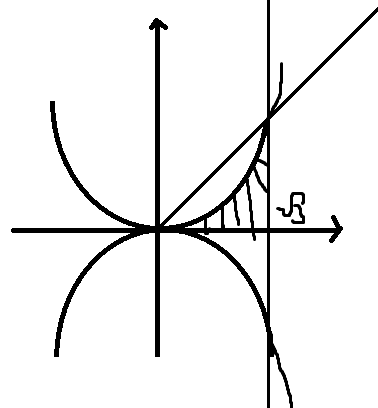
\includegraphics[width=\linewidth]{pics/pic4.png}
\end{minipage}

$$
s_{1 / 2}=\frac{1}{2} \int_0^{\pi / 3}(2 \tg \varphi )^2 \, d \varphi=\frac{1}{2} \cdot \varphi \int_0^{\pi / 3} \tg ^2
\varphi \, d \varphi=2 \int_0^{\pi / 3} \frac{\sin ^2 \varphi}{\cos ^2 \varphi} \, d \varphi= 
$$
$$
=2 \int_0^{\pi / 3} \frac{1-\cos ^2 \varphi}{\cos ^2 \varphi} \, d \varphi=2 \int_6^{\pi / 3} \frac{1}
{\cos^2 \varphi} \, d \varphi-2 \int_0^{\pi / 3} d \varphi= 
$$

$$
=\left.(2 \tg \varphi-2 \varphi)\right \biggr|_0 ^{\pi / 3}=2 \sqrt{3}-\frac{2 \pi}{3}=s_{1/2} \qquad  S=4 \sqrt{3}-\frac{4 \pi}{3} 
$$
\textbf{Ответ:} $S=4 \sqrt{3}-\frac{4 \pi}{3}$

\subsubsection*{Пункт б}
$$\left(\frac{x}{2}\right)^{2/3} + \left(\frac{y}{2}\right)^{2/3} = 1$$
\textbf{Решение:} \\
\begin{minipage}{0.6\textwidth}
$$\left(\frac{x}{2}\right)^{2 / 3}+\left(\frac{y}{2}\right)^{2 / 3}=1$$
$$
\begin{array}{c}
     \left(\frac{x}{2}\right)^{1 / 3}=\cos t \\
     \left(\frac{y}{2}\right)^{1 / 3}=\sin t
\end{array}
\quad
\left(\cos^2 t + \sin^2 t=1\right)
$$
\end{minipage}
\hfill
\begin{minipage}{0.3\textwidth}\raggedleft
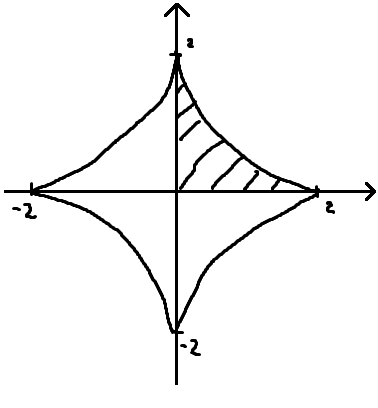
\includegraphics[width=\linewidth]{pics/pic5.png}
\end{minipage} 
$$
\begin{cases}
x=2 \cos ^3 t \\
y=2 \sin ^3 t 
\end{cases}
, ~t \in [0,2 \pi] \quad
\begin{cases}
y^{\prime}=6 \sin ^3 t \cos x \\
x^{\prime}=-6 \cos ^2 x \sin x 
\end{cases}
$$

$$
\frac{1}{4} s=\frac{1}{2} \int_0^{\pi / 2}\left(2 \cos ^3 t \cdot 6 \sin ^2 t \cos t+6 \cos ^3 t \sin t 2 \sin ^3 t\right)  \,d t= 
$$
$$
=\frac{1}{2} \cdot 12 \int_0^{\pi / 2}\left(\cos ^4 t \sin ^2 t+\sin ^4 t \cos ^2 t\right)\, d t= 6 \int_0^{\pi / 2}\left(\sin ^2 t \cos ^2 t\left(\cos ^2 t+1 \sin ^2 t\right)\right) \, d t=
$$
$$
=6 \int_0^{\pi / 2} \sin ^2 t \cos^2 t  \, d t=6 \cdot \frac{1}{4} \int_0^{\pi / 2} \sin ^2 2 t \, d t=\frac{3}{2} \int_0^{\pi / 2} \sin ^2 2 t \, d t= 
$$
$$
=\frac{3}{2} \int_0^{\pi / 2} \frac{1-\cos 4 t}{2} \, d t=\frac{3}{4} \int_0^{\pi / 2} \, dt -\frac{3}{4} \int_0^{\pi / 2} \cos 4 t \, d t= \frac{3}{4} \cdot \frac{\pi}{2} - \left.\frac{\sin 4 t}{4}\right\biggr|_0 ^{\pi / 2}=
$$
$$
=\frac{3}{32}\pi - \frac{\sin 2 \pi}{4} + 0 = \frac{3 \pi}{8} \qquad \frac{1}{4} s=\frac{3 \pi}{8} \quad \Rightarrow \quad s = \frac{9 \pi}{2}
$$
\textbf{Ответ:} $S = \cfrac{9\pi}{2}$
\newpage
\subsection*{Задача 3}
\subsubsection*{Пункт а}
$$
x=6-3 t^2, \quad y=4 t^3, x \geqslant 0
$$
\textbf{Решение:} 
$$
\begin{aligned}
& 6-3 t^2 \geq 0 \quad t^2 \leq 2, t \in[-\sqrt{2} ; \sqrt{2}] \\
& x^{\prime}=-6 t ; y^{\prime}=12 t^2 \quad 1 \quad i(x)^2+\left(y^{\prime}\right)^2=36 t^2+144 t^4=36 t^2\left(1+4 t^2\right) \\
& L=\int_{-\sqrt{2}}^{\sqrt{2}} \sqrt{x^2+y^{\prime 2}} d t=\int_{-\sqrt{2}}^{\sqrt{2}} \sqrt{36 t^2\left(1+4 t^2\right)} d t= \\
& =2 \int_0^{\sqrt{2}} 6 t \sqrt{1+4 t^2} d t=12 \int_0^{\sqrt{2}} t \sqrt{1+4 t^2} d t=6 \int_0^{\sqrt{2}} \sqrt{1+4 t^2} d t^2= \\
& =\frac{3}{2} \int_0^{\sqrt{2}} \sqrt{1+4 t^2} d\left(1+4 t^2\right)=\left.\left(1+4 t^2\right)^{\frac{3}{2}}\right|_0 ^{\sqrt{2}}=27-1=26
\end{aligned}
$$
\textbf{Ответ:} $26$
\subsubsection*{Пункт б}
$$y^3 = 3z, ~ 2yx = 1, ~ 1 \leq y \leq 3$$
\textbf{Решение:} \\
$$
\begin{aligned}
& y=t, \quad z=\frac{t^3}{3}, \quad x=\frac{1}{2 t}, \quad 1 \leq t \leq 3 \\
& x^{\prime}=-\frac{1}{2 t^2}, \quad y^{\prime}=1, \quad z^{\prime}=t^2 \\
& \left(x^{\prime}\right)^2+\left(y^{\prime}\right)^2+\left(z^{\prime}\right)^2=\frac{1}{4 t^4}+1+t^4=\left(\frac{1}{2 t^2}+t^2\right)^2 \\
& L=\int_1^3 \sqrt{x^{\prime^2}+y^{\prime 2}+z^{\prime 2}} d t=\int_1^3 \frac{1}{2 t^2}+t^2 d t=-\frac{1}{2 t}+\left.\frac{t^3}{3}\right|_1 ^3= \\
& =\left(-\frac{1}{6}+9\right)-\left(-\frac{1}{2}+\frac{1}{3}\right)=9+\frac{1}{2}-\frac{1}{6}-\frac{1}{3}=9 \qquad 
\end{aligned}
$$
\textbf{Ответ:} $9$ \newpage
\section*{Вариант 6}
\subsection*{Задача 2}
\subsubsection*{Пункт а}
$$r=\sqrt{\frac{\sin 3 \varphi}{\sin \varphi}}, r=4 \cos \varphi$$
\textbf{Решение:} 
$$
\begin{aligned}
& S_1=\frac{1}{2} \int_0^\pi \left(\sqrt{\frac{\sin 3 \varphi}{\sin \varphi}}\right)^2 \, d \alpha
=\frac{1}{2} \int_0^\pi \frac{\sin 3 \alpha}{\sin \alpha} \, d \alpha
=\frac{1}{2} \int_0^\pi \frac{3 \cos ^2 \alpha \sin \alpha-\sin ^3 \alpha}{\sin \alpha} d \alpha= \\
& =\frac{1}{2} \int_0^\pi 3 \cos ^3 \alpha \, d \alpha - \frac{1}{2} \int_0^\pi \sin ^2 \alpha \, d \alpha
=\frac{3}{2} \int_0^\pi \frac{\cos 2 \alpha+1}{2} \, d \alpha - \frac{1}{2} \int_0^\pi \frac{1-\cos 2 \alpha}{2} \, d \alpha= \\
& = \left | 
\begin{array}{c}
u = 2\alpha \\ d \alpha = \frac{d\varphi}{2}
\end{array}
\right | \quad \Rightarrow \quad \begin{cases}
    \frac{3}{2} \int_0^\pi \frac{\cos 2 \alpha+1}{2} \, d \alpha = \frac{1}{2} \int \frac{\cos \varphi}{2} \, d \varphi+\frac{1}{2} \int \frac{d \varphi}{2}=\frac{\sin 2 \alpha}{4}+\frac{\alpha}{2} \\
    \frac{1}{2} \int_0^\pi \frac{1-\cos 2 \alpha}{2} \, d \alpha= \frac{\alpha}{2}-\frac{\sin 2 \alpha}{4}
\end{cases} \\
& \left.S_1=\left(\frac{3}{2}\left(\frac{\sin 2 \alpha}{4}+\frac{\alpha}{2}\right)-\frac{1}{2} \frac{\alpha}{2}-\frac{\sin 2 \alpha}{\alpha}\right)\right)^\pi=\frac{\pi}{2} \\
& 2 S_2=\frac{1}{4} \int_0^{2 \pi} 16 \cos ^2 \alpha d \alpha=4 \int_0^{2 \pi} \frac{1+\cos 2 \alpha}{2} d \alpha=2 \cdot\left(\int_0^{0 \pi} d \alpha+\int_0^{2 \pi} \cos 2 \alpha d \alpha\right) \Rightarrow \\
& \Rightarrow S_2=2 \pi \\
& S_{\text{между ккривыми}}=2 \pi-\frac{\pi}{2}=\frac{3 \pi}{2}
\end{aligned}
$$
\textbf{Ответ:} $\cfrac{3\pi}{2}$
\subsubsection*{Пункт б}
$$x^{3}=a y^{4}-x^{2} y$$
\textbf{Решение:} \\
$$
\begin{aligned}
& x^{3}=a y^{4}-x^{2} y \quad\left\{\begin{array}{l}
x=r \cos \varphi \\
y=r \sin \varphi
\end{array}\right. \\
& r^{3} \cos ^{3} \varphi=a r^{4} \sin ^{4} \varphi-r^{2} \cos ^{2} \varphi r \sin \varphi \\
& r^{3} \cos ^{3} \varphi=r^{4} a \sin ^{4} \varphi-r^{3} \cos ^{2} \varphi \sin \varphi \mid: 2^{3} \\
& \cos ^{3} \varphi=r \operatorname{asin}^{4} \varphi-\cos ^{2} \varphi \sin \varphi \\
& \cos ^{2} \varphi \sin \varphi+\cos ^{3} \varphi=r \cdot a \sin ^{4} \varphi \\
\end{aligned}
$$

$$
r=\frac{\cos ^{2} \varphi \sin \varphi+\cos ^{3} \varphi}{a \sin ^{4} \varphi}
$$
\begin{center}
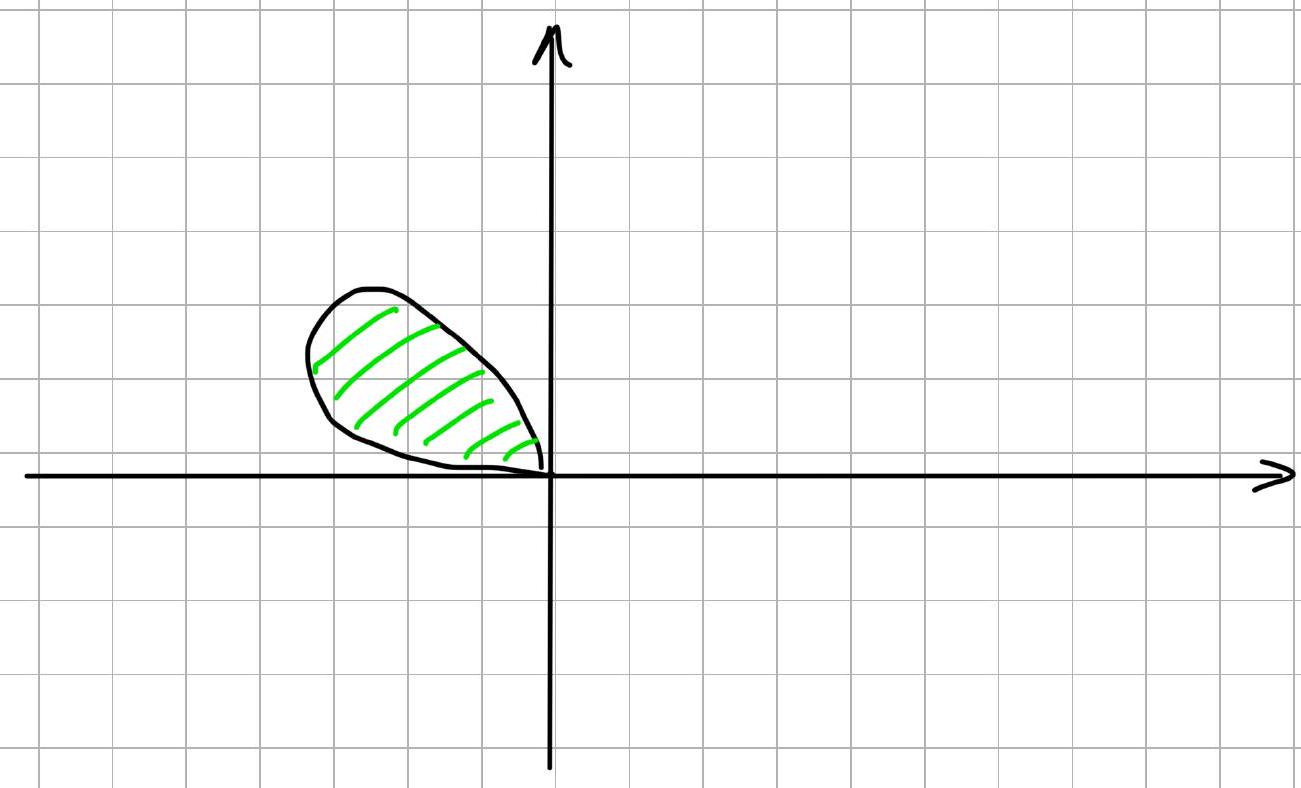
\includegraphics[scale=0.1]{pics/pic6.jpg}
\end{center}

$$
\begin{aligned}
& S=\int_{\varphi_{1} }^{\varphi_{2}} r^{2}(\varphi) d \varphi=\int_{\frac{\pi}{2}}^{\frac{3 \pi}{4}}\left(\frac{\cos ^{2} \varphi \sin \varphi+\cos ^{3} \varphi}{a \sin ^{4} \varphi}\right)^{2} d \varphi= \\
& =\quad \frac{1}{a^{2}} \int_{\frac{\pi}{2}}^{3 \frac{\pi}{4}} \frac{\operatorname{tg}^{2} \varphi+2 \operatorname{tg} \varphi+1}{\cos ^{2} \varphi+\operatorname{tg}^{8} \varphi} d \varphi=\left\{
\begin{array}{l}
u=2 \operatorname{tg} \varphi \\
d u=\frac{1}{\cos^{2} \varphi} d \varphi
\end{array}\right. \\
& =\frac{1}{a^{2}} \int \frac{32 u^{2}+128 u+128}{u^{8}} d u = \frac{1}{a^{2}} \int\left(\frac{32}{u^{6}}+\frac{128}{u^{7}}+\frac{128}{u^{8}}\right) d u= \\
&= -\frac{672 u^{2}+2240 u+1920}{105 a^{2} u^{7}} \text{ обратная замена}
\end{aligned}
$$

$$
\left.\left(-\frac{\operatorname{ctg}^{7} \varphi \operatorname{tg}^{2} \varphi}{\operatorname{5a}^{2}}-\frac{\operatorname{ctg}^{7} \varphi \operatorname{tg} \varphi}{3 a^{2}}-\frac{\operatorname{ctg}^{7} \varphi}{7 a^{2}}\right) \right \biggr|^{\frac{3 \pi}{4}}_{\frac{\pi}{2}} =\frac{1}{105 a^{2}}
$$

\textbf{Ответ}: $\frac{1}{105 a^{2}}$

\newpage
\subsection*{Задача 3}
\subsubsection*{Пункт а}
$$
x=6-3 t^3, y=\frac{9\left(2 t^2-t^4\right)}{8}, y \geqslant 0
$$
\textbf{Решение:} \\

$$
\begin{aligned}
& (\gamma)=\int_{T_0}^{T_1} \sqrt{\left(x^{\prime}(t)\right)^2+\left(y^{\prime}(t)\right)^2} d t \\
& x^{\prime}(t)=-9 t^2 \\
& y^{\prime}(t)=\frac{9}{2} t-\frac{9}{2} t^3
\end{aligned}
$$
Найдем промежутки:
$$
\begin{aligned}
& \frac{9\left(2 t^2-t^4\right)}{8} \geqslant 0 \Rightarrow \\
\Rightarrow & t \in[-\sqrt{2} ; \sqrt{2}]
\end{aligned}
$$
$$
\begin{aligned}
x^{\prime}(t)^2 & =M t^2 \\
y^{\prime}\left(t^2\right) & =\frac{11}{t^2}-\frac{81}{2} t^4+\frac{81}{4} t^6 \\
|\gamma| & =\int_{-\sqrt{2}}^{\sqrt{2}}\left(\frac{81}{2} t^4+\frac{81}{4} t^2+\frac{81}{4} t^6\right) d t=\left.\left(\frac{81 t^5}{10}+\frac{21 t^3}{4}+\frac{81 t^7}{28}\right)\right|_{-\sqrt{2}} ^2=\frac{4883 \sqrt{2}}{35}
\end{aligned}
$$
\textbf{Ответ:} $\cfrac{4883 \sqrt{2}}{35}$
\subsubsection*{Пункт б}
$$
z^3=12 x, \quad 2 z y=4, \quad
\frac{2}{3} \leqslant x \leqslant 18
$$
\textbf{Решение:} 
$$\text{Пусть } x = t ~ \Rightarrow ~ z = \sqrt[3]{12t}, \quad y = \cfrac{4}{2 \sqrt[3]{12t}}$$
$$
|y| = \int_{t_0}^{t_1 }\sqrt{(x^{\prime})^2 + (y^{\prime})^2 + (z^{\prime})^2 \, dt}
$$
Тогда $x^{\prime} = 1; \quad z^{\prime} = \cfrac{\sqrt[3]{12}}{3 \sqrt[3]{t^2}}; \quad y^{\prime} = - \cfrac{2 \sqrt[3]{18 t^2}}{9t^2}$
$$
\int_{\frac{2}{3}}^{18} \left(1 + \cfrac{\sqrt[3]{12}}{3 \sqrt[3]{t^2}} - \cfrac{2 \sqrt[3]{18 t^2}}{9t^2}  \right) \, dt = \int_{\frac{2}{3}}^{18} 1 \, dt + \int_{\frac{2}{3}}^{18} \cfrac{12^{1/3}}{3t^{2/3}} \, dt+ \int_{\frac{2}{3}}^{18} \cfrac{2 \cdot 18^{1/3}}{9 t^{4/3}} \, dt= 
$$
$$
\left. \left( t + \sqrt[3]{12t} + \cfrac{2 \sqrt[3]{18}}{3 \sqrt[3]{t}} \right) \right\biggr|^{18}_{\frac{2}{3}} = 22 \cfrac{2}{3}
$$
\textbf{Ответ:} $22 \cfrac{2}{3}$
\newpage
\section*{Вариант 8}
\subsection*{Задача 2}
\subsubsection*{Пункт а}
$$
r = 1 - 2 \cos 2 \varphi, ~ r = \cfrac{4 \sqrt{3}}{3} \sin \varphi$$
$$\left(r \geq 1 - 2 \cos 2 \varphi, ~ r \leq \cfrac{4 \sqrt{3}}{3} \sin \varphi \right)
$$
\textbf{Решение:}


\begin{minipage}{0.3\textwidth}
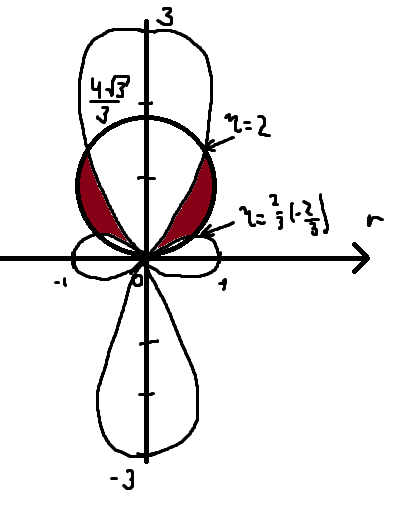
\includegraphics[width=\linewidth]{pics/pic1.png}
\end{minipage}
\hfill
\begin{minipage}{0.6\textwidth}\raggedleft
$r_1 = 1-2cos\varphi$ \\
$r_2 = \cfrac{4 \sqrt{3}}{3} \sin \varphi$
\end{minipage}

$$1 - 2 \cos 2\varphi = 1-2(1-2\sin^2 \varphi)\cfrac{4 \sqrt{3}}{3} \sin \varphi$$
$$4\sin^2 \varphi - \cfrac{4 \sqrt{3}}{3} \sin \varphi -1 = 0$$
$$\sin \varphi \frac{\frac{4\sqrt{3}}{3} \pm \sqrt{\frac{16}{3} + 16}}{8} =  \frac{4 \frac{\sqrt{3}}{3} \pm 8 \frac{\sqrt{3}}{3}}{8}$$
$$\varphi = \cfrac{\pi}{3} + 2\pi k \quad \varphi = \cfrac{2\pi}{3} + 2\pi k$$
$$\varphi = arcsin \left( - \cfrac{\sqrt{3}}{6}\right) + 2\pi k \quad \varphi = \pi - rcsin \left( - \cfrac{\sqrt{3}}{6}\right) + 2\pi k$$
\textbf{Проинтегрируем:}
$$S = 2 \cdot \frac{1}{2} \int_0^{\pi/3}\left( \cfrac{4 \sqrt{3}}{3} \sion \varphi \right)^2 - (1-2\cos 2\varphi)^2 \, d \varphi = \int_0^{\pi/3} \frac{16}{3} \sin^2 \varphi - (4 \sin^2 \varphi -1)^2 \, d \varphi =$$
$$ = \int_0^{\pi/3} -16 \sin^4 \varphi + \frac{40}{3} \sin^2 \varphi -1 \, d \varphi =  \int_0^{\pi/3} -16 \sin^2(1 - \cos ^2 \varphi) + \frac{40}{3} \sin^2 - 1 \, d \varphi =$$
$$=  \int_0^{\pi/3} (2 \sin 2\varphi)^2 - \frac{8}{3} \sin^2 \varphi -1 \, d \varphi = \left |
\begin{array}{c}
     1-2\sin^2 2\varphi = \cos 4 \varphi\\
     4 \sin^2 2\varpi = -2 \cos 4 \varphi + 2 \\
     -\frac{8}{3} \sin^2 \varphi = \frac{8}{6} (-2 \sin^2 \varphi) = \\ = \frac{8}{6}(1 - 2 \sin^2 \varphi) - \frac{8}{6}  =\frac{8}{6} \cos 2 \varphi - \frac{8}{6}
\end{array} 
\right| =
$$
$$
 =\int_0^{\pi/3}-2\cos 4 \varphi + \frac{8}{6} \cos 2 \varphi + 2 - \frac{4}{3} - 1 \, d \varphi = 
$$
$$
= \cfrac{- \sin 4 \varphi}{2} + \cfrac{2 \sin 2 \varphi}{3} - \cfrac{1}{3}\varphi \biggr | ^{\frac{\pi}{3}}_0 = \left( \cfrac{\sqrt{3}}{4} + \cfrac{\sqrt{3}}{3} - \cfrac{\pi}{9} \right) - 0 = \cfrac{7 \sqrt{3}}{12} - \cfrac{\pi}{9}
$$
\textbf{Ответ:} $\cfrac{7 \sqrt{3}}{12} - \cfrac{\pi}{9}$

\subsubsection*{Пункт б}
$$(x+y)^3=tx$$
\textbf{Решение:}
\begin{minipage}{0.3\textwidth}
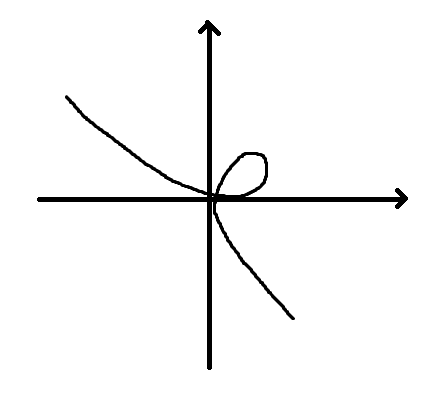
\includegraphics[width=\linewidth]{pics/pic2.png}
\end{minipage}
\hfill
\begin{minipage}{0.6\textwidth}\raggedleft
$$(x+y)^3=tx \quad y = tx $$
$$(x+tx)^3=2tx^2 \quad x^3(t+1)^3 = 2tx^2 \quad x(t+1)^3=2t$$
$$x = \cfrac{2t}{(t+1)^3}; ~ y = \cfrac{2t^2}{(t+1)^3}$$
\end{minipage}
$
\begin{aligned}
& x_t^{\prime}=\frac{2(t+1)^3-6 t(t+1)^2}{(t+1)^6}=\frac{2(t+1)-6 t}{(t+1)^4}=\frac{-4 t+2}{(t+1)^4} \\
& y_t^{\prime}=\frac{4 t(t+1)^3-6 t^2(t+1)^2}{(t+1)^6}=\frac{4 t(t+1)-6 t^2}{(t+1)^4}=\frac{-2 t^2+4 t}{(t+1)^4} \\
& S=\frac{1}{2} \int_0^{+\infty}\left|y \cdot x^{\prime}-x y^{\prime}\right| d t=\frac{1}{2} \int_0^{+\infty} \frac{2 t^2 \cdot 2 \cdot(-2 t+1)}{(t+1)^7}-\frac{2 t \cdot 2 t \cdot(t+2)}{(t+1)^7} \mid d t= \\
&= 2 \int_0^{+\infty}\left(\frac{t^2}{(t+1)^7}(-2 t+1+t-2) \mid d t=\int_0^{+\infty} \frac{t^2}{(t+1)^6} d t\right. \\
&= \int_0^{+\infty} \frac{t^2+2 t+1}{(t+1)^6}-\frac{2 t+2}{(t+1)^6}+\frac{1}{(t+1)^6} d t=2 \int_0^{+\infty}(t+1)^{-4}-2(t+1)^{-5}+\left(t+y^6 d t=\right. \\
&= \frac{2(t+1)^{-3}}{-3}-\frac{4(t+1)^{-4}}{-4}+\left.\frac{2(t+1)^{-5}}{-5}\right|_0 ^{+\infty}= \\
&=-\frac{2}{3(t+1)^3}+\frac{1}{(t+1)^4}-\left.\frac{2}{5(t+1)^5}\right|_0 ^{+\infty}=\left.\frac{-10(t+1)^2+15(t+1)-6}{15(t+1)^5}\right|_0 ^{+\infty} \\
&=-\frac{-10+15-6}{15}=\frac{1}{15}
\end{aligned}
$
\textbf{Ответ:} $\cfrac{1}{15}$.

\subsection*{Задача 3}
\subsubsection*{Пункт а}
$$x=2\cos^3 t, ~ y = 3\sin^3 t$$
\textbf{Решение:} \\
\begin{minipage}{0.3\textwidth}
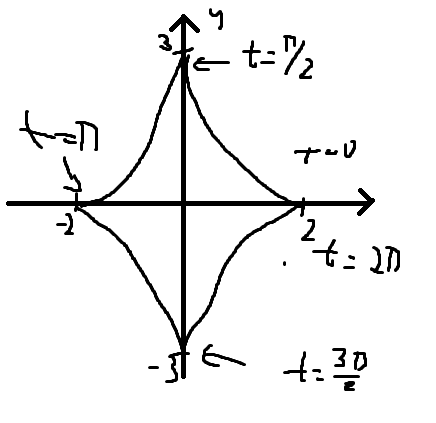
\includegraphics[width=\linewidth]{pics/pic3.png}
\end{minipage}
\hfill
\begin{minipage}{0.6\textwidth}\raggedleft
$$
x^{\prime} = 2 \cdot 3 \cdot (-\sin t) \cdot \cos^2 t
$$
$$
y^{\prime} = 9 \cos t \cdot \sin ^2 t
$$
\end{minipage}

$$
L = \int^{2\pi}_0 \sqrt{(s^{\prime})^2 + (y^{\prime})^2} \, d t= 4 \int^{\frac{\pi}{2}}_0 3 \cdot \sin t \cdot \cos t \sqrt{4 \cos^2 t + 9 \sin ^2 t} \, dt = 
$$
$$
= 
\left|
\begin{array}{l}
4 \cos^2 t + 9 \sin^2 t = x \\
-8\sin t \cos t + 18 \sin t \cos t \, dt = dx \\
10 \sin t \cos t \, d t=d x \\
t=\frac{\pi}{2} \quad x=9 \\
t=0 \quad x=4
\end{array} \right| =\frac{6}{5} \int_4^9 \sqrt{x} d x=
$$
$$
=\left.\frac{6}{5} \cdot \frac{2}{3}(\sqrt{x})^3\right|_4 ^9
 =\frac{4}{5}(27-8)=15,2 
$$

\textbf{Ответ:} $15,2$

\subsubsection*{Пункт б}
$$\delta] z^2=2 x, x z=3 y \quad 0 \leqslant x \leqslant 8 $$
\textbf{Решение:} \\
$
\begin{aligned}
& z=6 t, x=18 t^2 \quad y=36 t^3 \\
& 0 \leqslant 18 t^2 \leqslant 8 \quad 0 \leqslant t^2 \leqslant \frac{4}{9} \quad t \in\left[-\frac{2}{3} ; \frac{2}{3}\right] \\
& \left(x^{\prime}\right)^2+\left(y^{\prime}\right)^2+\left(z^{\prime}\right)^2=(36 t)^2+\left(108 t^2\right)^2+36= \\
& =36^2 \cdot t^2+36^2 \cdot 9 \cdot t^4+36=36^2\left(9 t^4+t^2+\frac{1}{36}\right)=36^2\left(3 t^2+\frac{1}{6}\right)^2 \\
& L=\int_{-\frac{2}{3}}^{\frac{2}{3}} \sqrt{x^{\prime 2}+y^2+z^{\prime 2}} d t=\int_{-2 / 3}^{2 / 3} 36\left(3 t^2+\frac{1}{6}\right) d t=108 \int_{-2 / 3}^{2 / 3} t^2+6 \int_{-2 / 3}^{2 / 3} 1 d t= \\
&=\left.72 t^3\right|_0 ^{2 / 3}+\left.12 t\right|_0 ^{2 / 3} =72 \cdot \frac{8}{27}+8=\frac{64}{3}+8 \qquad \textbf{Ответ:} ~ \cfrac{64}{3} + 8
\end{aligned}
$ 